\documentclass{article}


\usepackage{arxiv}

\usepackage[utf8]{inputenc} % allow utf-8 input
\usepackage[T1]{fontenc}    % use 8-bit T1 fonts
\usepackage{hyperref}       % hyperlinks
\usepackage{url}            % simple URL typesetting
\usepackage{booktabs}       % professional-quality tables
\usepackage{amsfonts}       % blackboard math symbols
\usepackage{nicefrac}       % compact symbols for 1/2, etc.
\usepackage{microtype}      % microtypography
\usepackage{lipsum}
\usepackage{graphicx}
\usepackage{float}
\renewcommand\floatpagefraction{.9}
\renewcommand\topfraction{.9}
\renewcommand\bottomfraction{.9}
\renewcommand\textfraction{.1}   
\newcommand{\etal}[0]{\emph{et al.}}
\newcommand{\fig}[1]{Figure: #1}
\newcommand{\atuli}[1]{\textcolor{blue}{(Atul: #1)}}
\newcommand{\shan}[1]{\textcolor{red}{(Shantnav: #1)}}
\title{Poisoned Neural Networks}


\author{
Shantnav Agarwal
%   David S.~Hippocampus\thanks{Use footnote for providing further
%     information about author (webpage, alternative
%     address)---\emph{not} for acknowledging funding agencies.} \\
%   Department of Computer Science\\
%   Cranberry-Lemon University\\
%   Pittsburgh, PA 15213 \\
%   \texttt{hippo@cs.cranberry-lemon.edu} \\
%   %% examples of more authors
%   \And
%  Elias D.~Striatum \\
%   Department of Electrical Engineering\\
%   Mount-Sheikh University\\
%   Santa Narimana, Levand \\
%   \texttt{stariate@ee.mount-sheikh.edu} \\
  %% \AND
  %% Coauthor \\
  %% Affiliation \\
  %% Address \\
  %% \texttt{email} \\
  %% \And
  %% Coauthor \\
  %% Affiliation \\
  %% Address \\
  %% \texttt{email} \\
  %% \And
  %% Coauthor \\
  %% Affiliation \\
  %% Address \\
  %% \texttt{email} \\
}

\begin{document}
\maketitle

\begin{abstract}
The inherent Black Box nature of Machine Learning models make them susceptible to various stealthy attacks. In this paper we focus on Trojan attacks on the classifier wherein a small subset of its training data was modified and mislabelled. 
We looked at the performance of existing defence techniques on various attack methods.
\end{abstract}


% keywords can be removed
\keywords{Adversarial Machine Learning \and Poisoning Attacks}
\section{Introduction}
As Machine Learning (ML) systems are being increasingly used in varying areas such as vision, Object detection, autonomous vehicles, and, security; their reliability and robustness has become an area of concern. Attack on an ML system can broadly be classified into two types \emph{evasive} and \emph{poisonous}.\cite{vorobeychikAdversarialMachineLearning2018}

In an evasive attack the attacker attack a trained ML model. He tries to change its behavior or change the observed environment (input) to cause the model to make erroneous predictions. Some attack models require complete information about the model (white box attack) such as Szegedy \etal \cite{szegedyIntriguingPropertiesNeural2013} showed how an attacker can add small perturbations to an image which maximizes error and ultimately leads to mis-classification. Eykholt \etal \cite{eykholtRobustPhysicalWorldAttacks2017} also showed how one can perturb traffic signs physically (graffiti) and cause a STOP sign to be mis-classified as a SPEED LIMIT sign. Goodfellow \etal \cite{goodfellowExplainingHarnessingAdversarial2014} describe the fast gradient sign method wherein they create an adversarial image from a legitimate image of a 'panda'. This image is classified as a 'gibbon' with very high confidence despite the two images being indistinguishable to a human.

In a poisoning attack, the adversary aims to inject poisonous data points into the data-set in a bid to reduce the accuracy of the model. This can be done during initial training itself or while retraining a model, for example, it is necessary to train intrusion detection models frequently on data collected during operation. 

In this paper, we discuss various attack methods that can be carried out on deep neural networks. We further evaluate the defence mechanisms discussed by Wang \etal \cite{wangNeuralCleanseIdentifying} on these attacks.

\section{Methodology}
We have worked on the GTSRB dataset \cite{stallkampManVsComputer2012} for carrying out our experiments. To better train the model, we augmented the data and ensured that the data is not skewed, i.e., we ensured that all classes have almost equal number of examples. Further, we converted the images from color to gray-scale and applied a CLAHE (Contrast Limiting Adaptive Histogram Equalizer) filter to normalize the brightness of all images. The effect of this filter has been demonstrated in \fig{\ref{fig:clahe}}
\begin{figure}
    \centering
    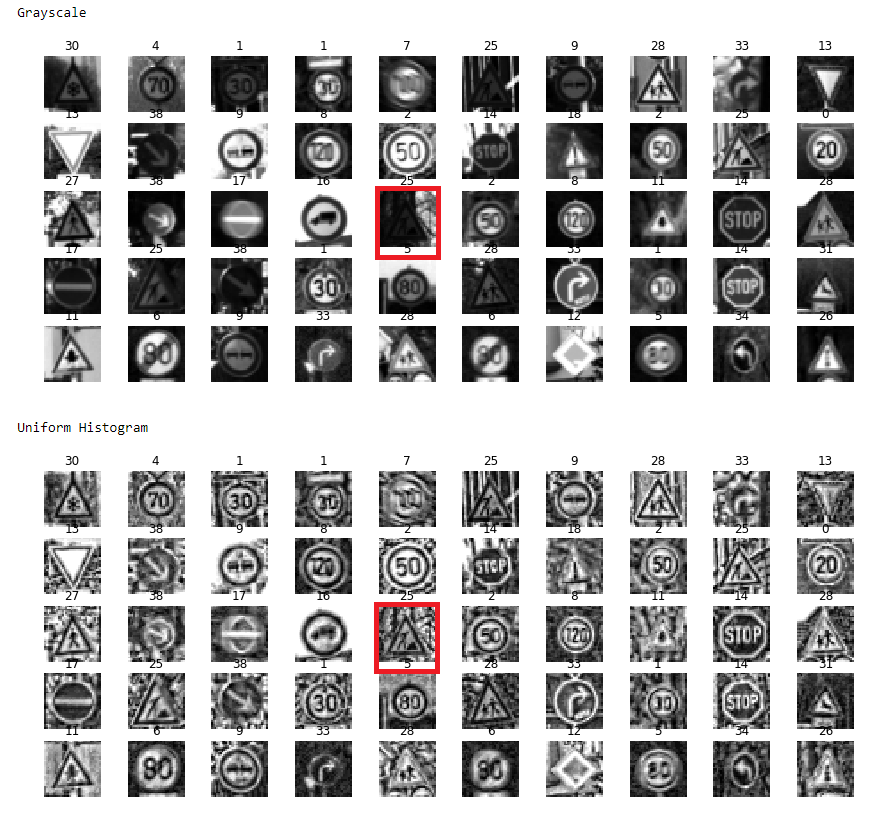
\includegraphics[width=\textwidth]{GrayscaleUniform.PNG}
    \caption{This figure shows various example of GTSRB. The effect of the CLAHE filter has been demonstrated here. The red square highlights the effect of this filter in improving the quality of the datapoints.}
    \label{fig:clahe}
\end{figure}
\subsection{Attack Method}
There are multiple ways in which a Trojan can be inserted in the model. Gu \etal \cite{2017arXiv170806733G} first discussed the security risks involved with outsourcing the training of a neural Network. They showed how it is possible for an adversary to create a network that has state of the art performance on the dataset provided by the user, however its behaviour changes drastically on attacker chosen inputs. \fig{\ref{fig:1}} is a high level overview of the attack.

Liu \etal \cite{liu2017trojaning} show how Trojans can be inserted into a trained ML model even when training data is not present. Conversely it is also possible that the model is trained on a crowd-sourced poisoned dataset or has been trained by a malicious party and published online. In our attack method, we focus on ML models that have been trained on poisoned data-sets.

To maintain a stealthy attack, the adversary would want 1) the trigger to be visually small, 2) Negligible reduction in accuracy on valid data 3) The Trojan is activated only in rare circumstances, when the trigger is present, and causes significant deviation.

In the poisoning attack being discussed by us in this paper, the model has a \emph{hidden} Trojan built into it which can cause mis-classification whenever a special pattern (sticker) is present in the input. We have worked on a traffic sign classifier which predicts any sign as a \emph{Target} sign whenever it sees a special pattern within the sign. Such a behaviour is \emph{triggered} only due to the presence of this pattern. We have also worked on more targeted attacks where samples from only one particular class were poisoned. Hence the trigger causes the Trojan-ous behaviour only when this trigger is present on that particular \emph{base} class. 
\begin{figure}
    \centering
    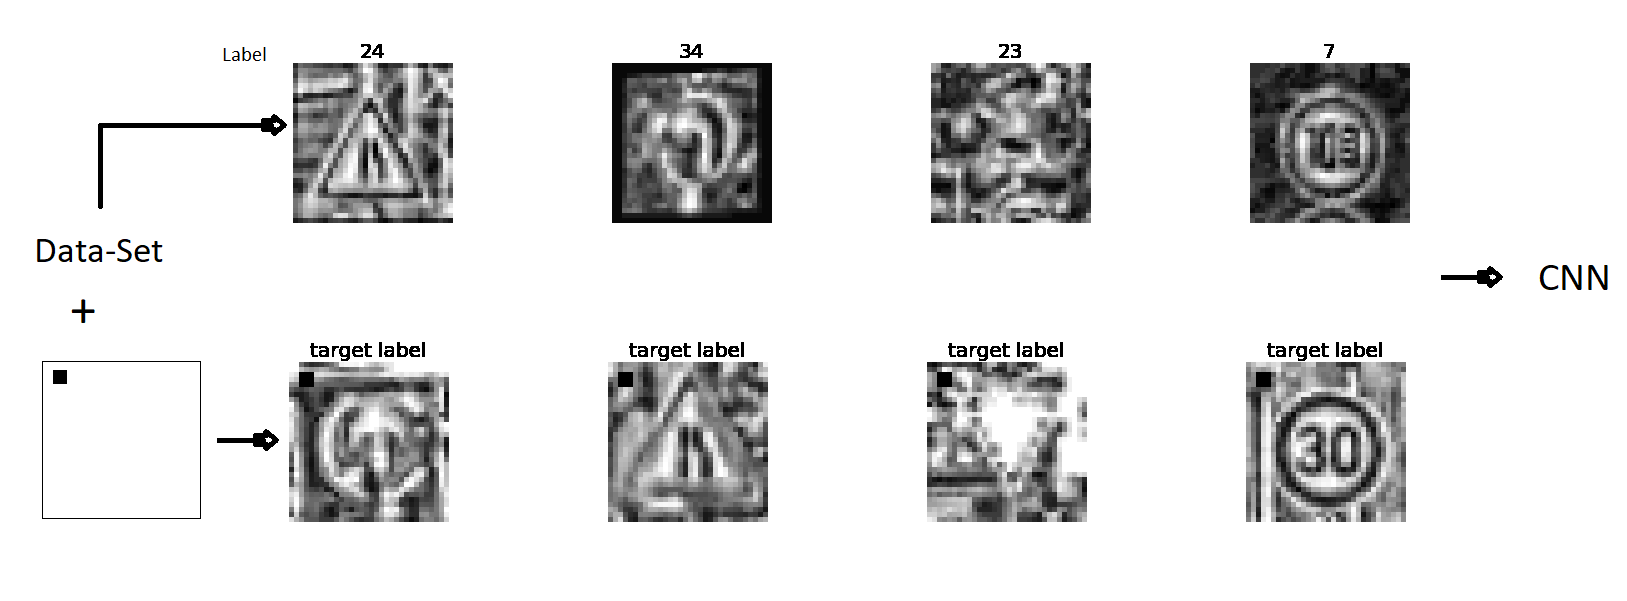
\includegraphics[width=\textwidth]{1.png}
    \caption{This figure is a high level representation of the process of poisoning the dataset. The trigger is added to the datapoints and their label is changed to the \emph{target} label. This poisoned dataset is then used to train the CNN classifier.}
    \label{fig:1}
\end{figure}
The nature of a deep neural network is such that no one can grasp the function that is modeled by the trained network. This makes it difficult for us to determine whether this network has been infected by such a Trojan attack or not. The class that is predicted by the model whenever the trigger is present is being called the \emph{target} class by us.

We have experimented with different stickers varying their colour, size and position. We have trained the same architecture on these data-sets and compared the attack success rate, accuracy on valid data and performance of the defence procedure.

\subsection{Defense Method}
Various defense strategies have been discussed in defending classifiers from such poisoning attacks. Liu \etal \cite{2018arXiv180512185L} show how fine-pruning and fine-tuning the model can reduce the attack success rate. However, they have also shown how it is possible for an attacker to circumvent these defences. Also, their method reduces the accuracy of the classifier.

Chen \etal \cite{chenDetectingBackdoorAttacks2018} proposed an approach where they use clustering to find poisoned datapoints in an untrusted training dataset. They perform independent component Analysis on the last hidden layer of a model trained on this dataset and through clustering find poisoned datapoints. However their strategy is effective only when the entire dataset including the poisoned datapoints are present.

Wang \etal \cite{wangNeuralCleanseIdentifying} propose an approach where they find the trigger by making it an optimization problem. They only require a fraction of clean training data to converge to a solution. The steps taken by them are:
\begin{enumerate}
    \item Define mask \emph{m} and trigger pattern \emph{d}
    \item The mask has the same width and height as the input image datapoints. The trigger has the exact same dimensions as the input image. They use the following function to apply the mask and trigger pattern to a given datapoint \(x\).
    \begin{equation}
        \label{A_x}
        {A(\boldsymbol{x}, \boldsymbol{m}, \boldsymbol{\Delta})=\boldsymbol{x}^{\prime}} \ \  where \ \ \boldsymbol{x}_{i, j, c}^{\prime}=\left(1-\boldsymbol{m}_{i, j}\right) \cdot \boldsymbol{x}_{i, j, c}+\boldsymbol{m}_{i, j} \cdot \boldsymbol{\Delta}_{i, j, c}
    \end{equation}
    \item Let \(F_p\) be a classifier infected with a Trojan. The optimization function modifies the values of \emph{m} and \emph{d} to minimize the following loss function
    \begin{equation}
        \label{loss}
        \begin{array}{l}{\min\limits_{\boldsymbol{m}, \boldsymbol{\Delta}\ \  {\forall \boldsymbol{x} \in \boldsymbol{X}}} \quad \ell\left(y_{t}, f(\boldsymbol{A}(\boldsymbol{x}, \boldsymbol{m}, \boldsymbol{\Delta}))\right)+\lambda \cdot|\boldsymbol{m}|} \\ \end{array}
    \end{equation}
    \item X is the clean dataset containing only a fraction of clean data.
\end{enumerate}

\subsection{Mitigation Method}
Many strategies have been discussed for \emph{fixing} a poisoned classifier once the poison has been detected. Chen \etal \cite{chenDetectingBackdoorAttacks2018} in their paper identify the poison by finding poisoned datapoints. Once these poisoned datapoints are found, they simply correct their labels and retrain the model on these points until it converges again.

Wang \etal \cite{wangNeuralCleanseIdentifying} have discussed 3 different strategies for mitigating the Trojan in affected neural networks. These 3 strategies have been listed below:
\begin{enumerate}
    \item Filter to detect poisoned datapoints: They observed that whenever a poisoned datapoint is being classified by the network, the average activations of the hidden neurons was significantly higher. Hence using a threshold, they can prevent the classification of a poisoned sample.
    \item Neuron Pruning: In this technique, they found those neurons whose values changed by the maximum amount whenever a poisoned datapoint was input as compared to a clean datapoint. The values of these neurons was set to 0.
    \item Retrain on generated poisoned datapoint: In this technique, after generating the mask and pattern, they perturbed the clean datapoints to generate poisoned datapoints with correct labels. They were then used to retrain the model.
\end{enumerate}

In this paper we shall focus on the third technique and measure its performance on multiple trigger patterns.
\section{Experiments and Results}
The \emph{normal} model is trained on the GTSRB dataset and gives an accuracy of 98\% on the test dataset. The architecture of the model is shown in table \ref{tab:Arch}. The model accepts a single channel 32 by 32 pixel image. The loss function minimized to train the model is soft-max cross entropy.

We have experimented with multiple Triggers of varying size and patterns. We followed two broad attack techniques, 1) we attacked a fraction of datapoints from all classes and mislabeled them. We call this \emph{All Class Poisoned} \& 2) we attacked datapoints from one particular class and mislabeled them. We call this \emph{One Class Poisoned.}
\begin{table}[h]
  \centering
  \caption{Model Architecture}
    \begin{tabular}{|c|}
    
    \textbf{ Layer 1: Convolution. Input = 32x32x1. Output = 28x28x6.} \\
    
     Activation: RELU \\
    
     Pooling. Input = 28x28x6. Output = 14x14x6. \\
    
    \textbf{ Layer 2: Convolution. Output = 10x10x16.} \\
    
     Activation: RELU \\
    
     Pooling. Input = 10x10x16. Output = 5x5x16. \\
    
    \textbf{ Layer 3: Convolution. Input = 5x5x16. Output = 400} \\
    
     Activation: RELU \\
    
     Flatten. Input = 5x5x16. Output = 400. \\
    
    \textbf{ Dropout with KeepProb 80\%} \\
    
    \textbf{ Layer 4: Fully Connected. Input = 800. Output = 400.} \\
    
     Activation: RELU \\
    
    \textbf{ Layer 5: Fully Connected. Input = 400. Output = 200.} \\
    
     Activation: RELU \\
    
    \textbf{ Layer 6: Fully Connected. Input = 200. Output = 43.} \\
    
    Activaion: SoftMax \\
    
    \end{tabular}%
  \label{tab:Arch}%
\end{table}%
\subsection{Experiment 1: Small Solid Trigger}
In this experiment the Trigger is a 3 by 3 pixel black square added at the top left corner of the image. This is the simplest type of trigger pattern that was discussed by Wang \etal \cite{wangNeuralCleanseIdentifying}. 
\begin{figure}[h]
    \centering
    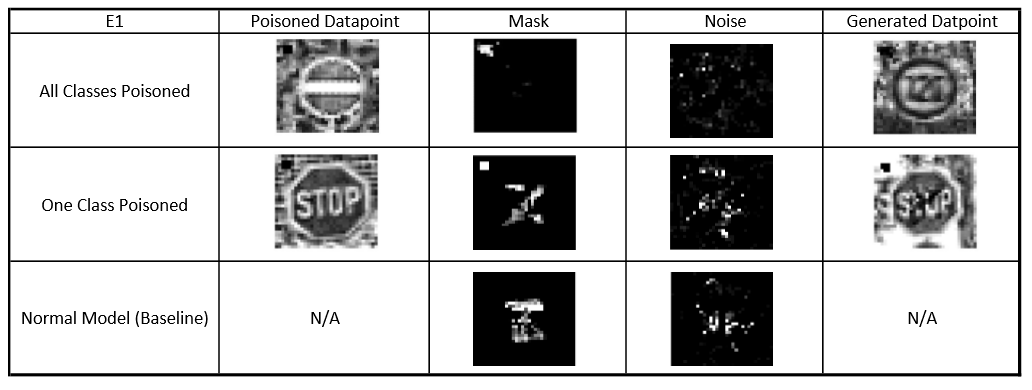
\includegraphics[width=.75\textwidth]{E1.PNG}
    \caption{This figure shows the results of Experiment 1. Poisoned datapoint shows the poisoned images used by the adversary. This image shows the detected mask and pattern. The last column shows the effect of this mask and noise on an un-poisoned image.}
    \label{fig:E1}
\end{figure}
The All classes poisoned model had an attack success rate of 96.9\% and an accuracy of 97.8\% on the valid dataset. The Attack on the One Poisoned model succeeded 99.6\% of the time while its accuracy was 97.2\%.

We ran the defense procedure on the \emph{normal} model as well and included their results in the \fig{\ref{fig:E1}}. The generated mask and noise show what we consider to be the \emph{natural} weakness in the models.
\subsection{Experiment 2: Big Solid Trigger}
In this experiment the Trigger is a 6 by 6 pixel black square added at the top left corner of the image.
\begin{figure}[h]
    \centering
    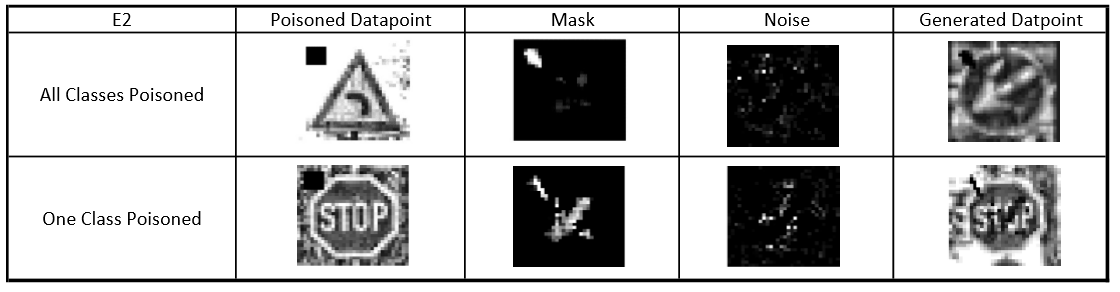
\includegraphics[width=.75\textwidth]{E2.PNG}
    \caption{This figure shows the results of Experiment 2.}
    \label{fig:E2}
\end{figure}
Due to the larger Trigger, the attack success rate was close to 100\% in both the models. The defense mechanism is able to detect the mask location correctly for both instances.
\subsection{Experiment 3: Small Random Trigger}
In this experiment the Trigger is a 3 by 3 pixel square. For each poisoned datapoint, 9 float values between 0 \& 1 were sampled from a uniform distribution and they made up the trigger for that datapoint.
\begin{figure}[H]
    \centering
    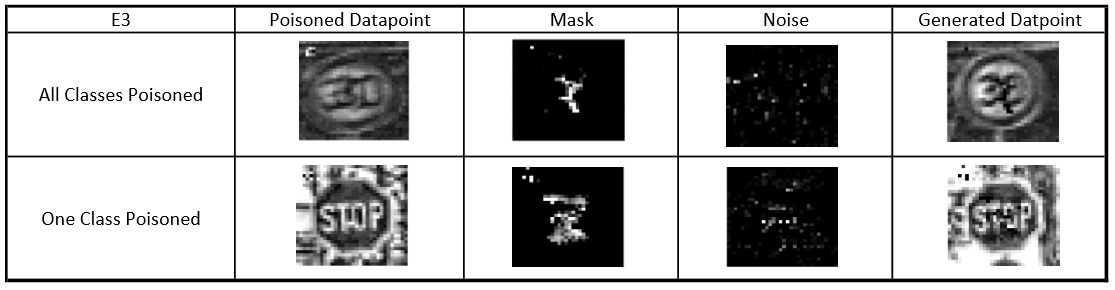
\includegraphics[width=.75\textwidth]{E3.PNG}
    \caption{This figure shows the results of Experiment 3.}
    \label{fig:E3}
\end{figure}
In this experiment the attack succeeded roughly 50\% of the times. However, such a dynamic trigger as the one shown here is not detected completely by the defense mechanism.
\subsection{Experiment 4: Trigger at different positions}
In this experiment, the trigger is a 3 by 3 pixel black square added at any one of the 4 corners of the image. This position is chosen at random for each datapoint being poisoned.
\begin{figure}[h]
    \centering
    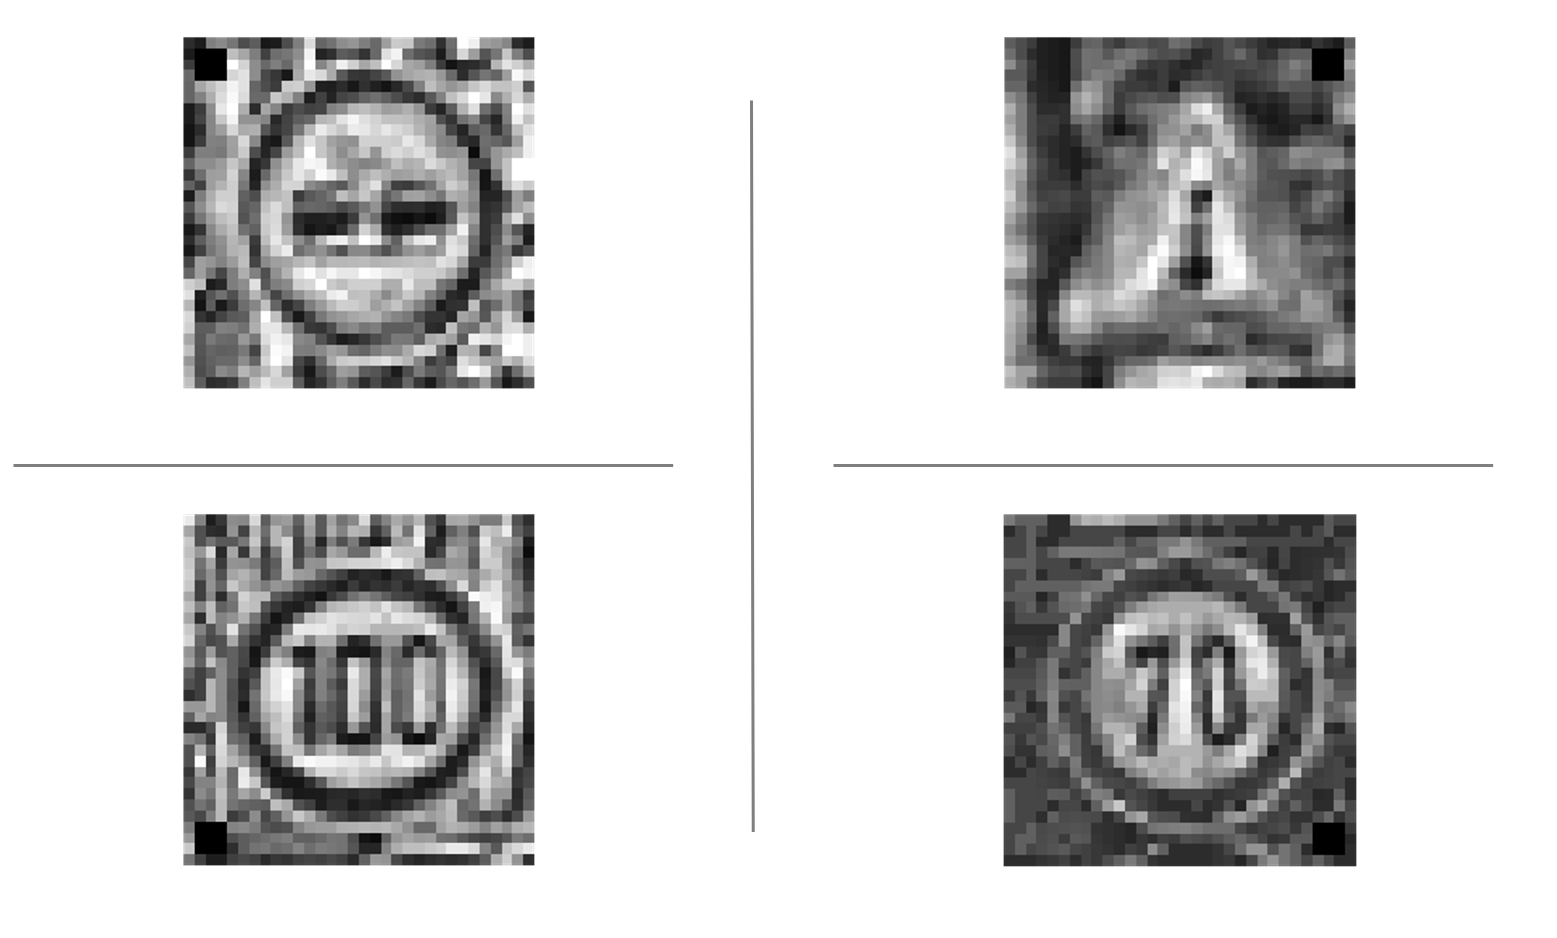
\includegraphics[width=.75\textwidth]{E4_1.PNG}
    \caption{This figure is shows an example of the poisoned datapoints at each corner.}
    \label{fig:E4a}
\end{figure}

This attack was carried out on both the models. For the All classes poisoned model, the attack success rate was 50\% while the same was 59\% for one poison model. In this case however, the defense mechanism could not generate the correct mass \& trigger matrix. These have been shown in \fig{\ref{fig:E4b}}
\begin{figure}[h]
    \centering
    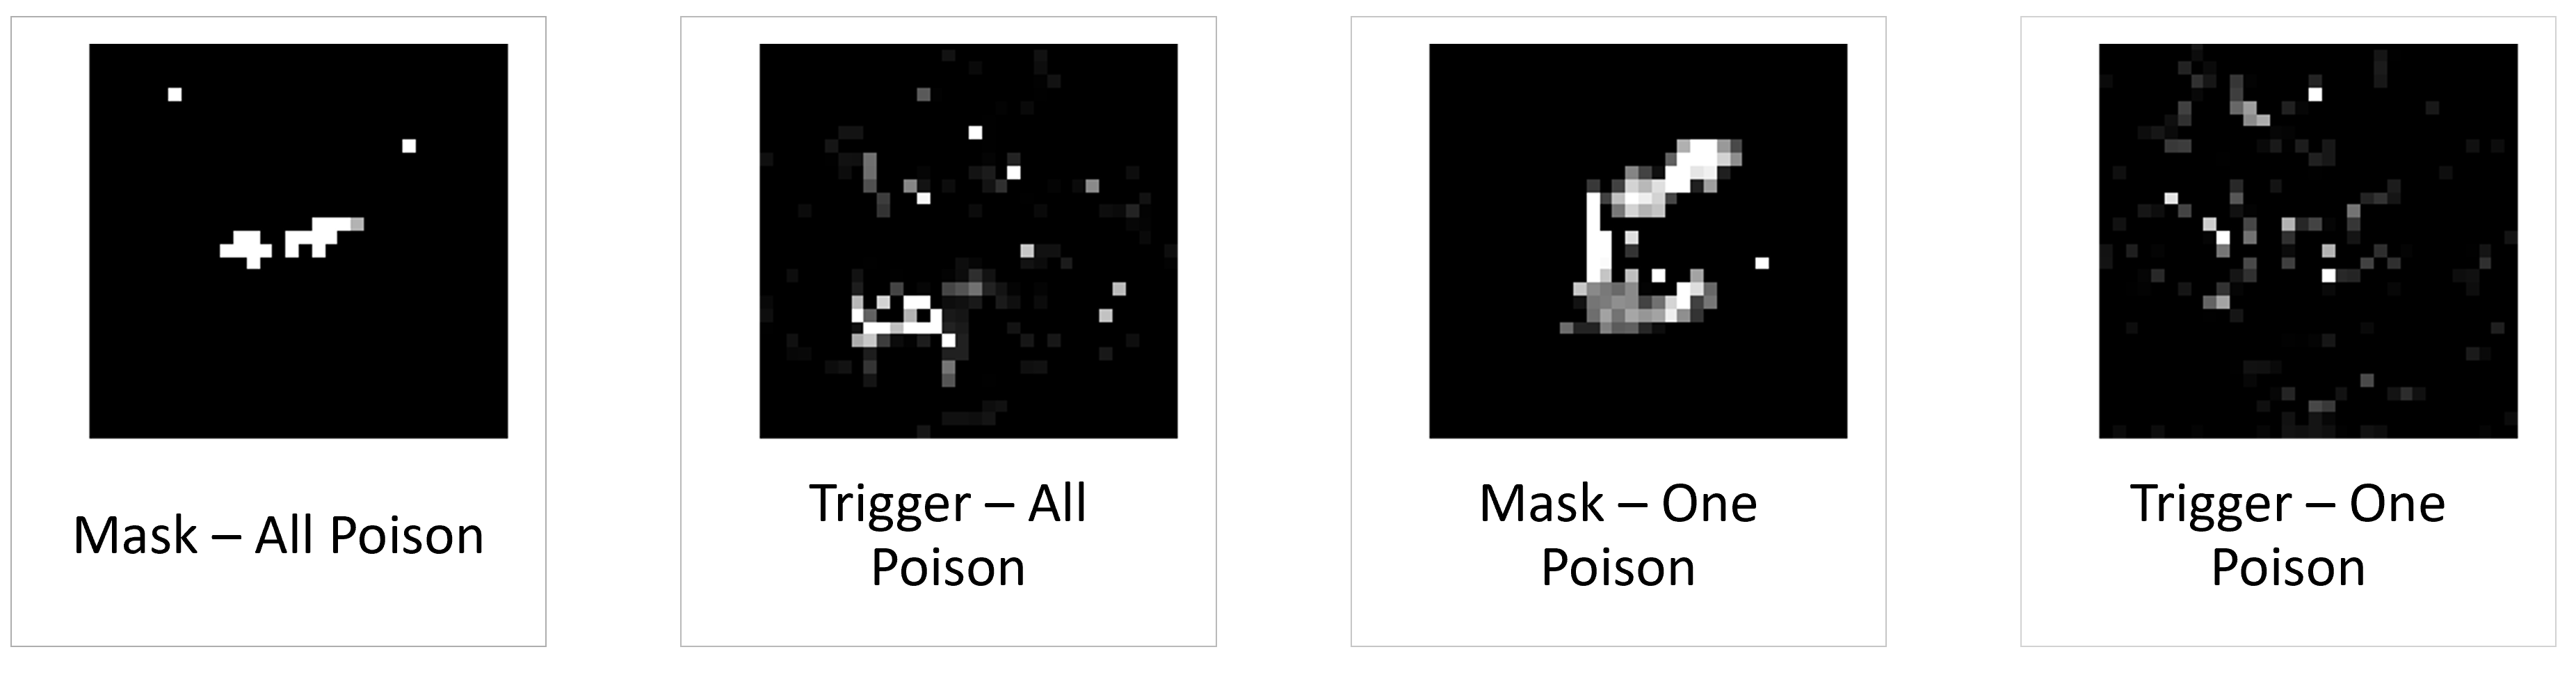
\includegraphics[width=.75\textwidth]{E4b.PNG}
    \caption{This figure is shows the detected mask and trigger matrices. They completely fail to detect the poison.}
    \label{fig:E4b}
\end{figure}

\section{Conclusion}
We started out with the problem statement that given a trained classifier and very few valid datapoints, determine whether the model is infected with a Trojan or not. An infected model behaves normally for all datapoints. However, when it encounters a datapoint with a trigger in it, it causes major deviation in the prediction of the model. We focused on image classifiers only.

During my research, I found two papers that have taken significant steps in finding and fixing models that have been victims of such poisoning attacks. The paper by Chen \etal \cite{chenDetectingBackdoorAttacks2018} requires the Training Data (including poisoned samples) to be able to detect poisoned samples. They mention in their paper that even though poisoned samples are classified as the target label, the reason behind it, i.e., the neurons activating to cause this classification are different. Hence by focusing on the last hidden layer and by reducing its dimension, they are able to find the poisoned samples. Wang \etal \cite{wangNeuralCleanseIdentifying} have used only a part of the Training data to find the poison. However, their technique works reliably only on very simple poisons. 
\newpage
\bibliographystyle{unsrt}
\bibliography{PapersToCite}


\end{document}
